\section{数字成形与能量估计}\label{sec:5-3}

在低能核物理与在束 $\gamma$ 谱学实验中，探测器测得的特征 $\gamma$ 跃迁能量与谱峰面积，是确定核能级位置、跃迁多极性与绝对跃迁几率 $B(XL)$ 的实验输入。然而，本节以半导体探测器为例：能量沉积首先产生载流子，电荷运动与前置放大器将其转化为波形；闪烁探测器还包含光产生及光电转换等环节。传统的模拟核电子学通过电阻、电容与放大器构建模拟成形网络来获取脉冲幅度；而在现代数字化数据获取系统中，前置放大器输出信号由高速模数转换器（ADC）直接进行均匀离散时间采样，将连续波形转化为离散序列~\cite{wu-hongyi-2020-general-purpose-digital-daq-thesis, wu-2021-general-purpose-digital-daq-waveform-analysis}。

这一技术转换使得能量提取能够通过离散滤波算法在数字信号处理器或可编程逻辑门阵列（FPGA）中灵活实现。然而，数字成形并非简单执行数学平滑，其离散递推结构、极零消除匹配、平顶时间参数以及堆积判弃逻辑，直接决定了能谱的分辨率、峰位稳定性与有效计数率响应。若对算法环节的物理机制与响应边界缺乏清晰把握，测得的峰面积与强度比值便可能掺入仪器响应偏差。本节从探测器电荷积分波形出发，系统推导离散梯形滤波与极零消除递推算法，分析平顶成形对弹道亏损的缓解效果与物理边界，并讨论基线扰动及堆积判弃对核谱学能量与强度的系统性影响。

\subsection{探测器电荷收集与前放信号的物理生成}\label{subsec:5-3-1}

半导体探测器记录 $\gamma$ 射线的初始物理过程是带电次级粒子在晶体中的电离能量损失。当入射能量为 $E_\gamma$ 的光子在晶体内完全沉积其能量时，在理想完整收集条件下，单个读出电极所对应的收集电荷绝对值可写为：
\begin{equation}\label{eq:5-3-q0}
Q_0 = \frac{e E_\gamma}{\epsilon},
\end{equation}
其中 $e$ 为元电荷，$\epsilon$ 为探测介质中平均产生一对电子-空穴对所需的电离能量。关于具体探测器的电荷输运与探测物理，将在第~5.2~节展开讨论。

在工作电场下，电子和空穴漂移并在读出电极上诱导电流。相互作用位置、漂移路径与收集过程的差异，使脉冲前沿具有有限且变化的持续时间。具体输运与电极响应留在第~5.2~节；这里关心这种前沿差异怎样进入数字能量估计。

感应电荷随后进入电荷灵敏前置放大器（CSPA）。前置放大器利用反馈积分电容 $C_f$ 积分输入电流，并在输出端产生阶跃电压脉冲；同时，并联的反馈电阻 $R_f$ 提供直流泄放通道，使电荷缓慢释放，形成长指数衰减尾部。考虑载流子收集过程引入的有效上升时间参数 $\tau_r$ 与前放反馈衰减时间常数 $\tau_d = R_f C_f$，前放输出的模拟电压脉冲可唯象描述为：
\begin{equation}\label{eq:5-3-vt}
v(t) = \frac{Q_0}{C_f} \left(1 - e^{-t/\tau_r}\right) e^{-t/\tau_d} \, u(t),
\end{equation}
其中 $u(t)$ 为连续时间单位阶跃函数。为了抑制前放反馈电阻带来的并联热电流噪声，通常需要选取阻值很大的反馈电阻，这使得衰减时间常数 $\tau_d$ 显著长于脉冲上升沿。在在束核物理实验中，当事件计数率较高时，相继到达的脉冲往往叠加在先前脉冲尚未完全衰减的长尾上，产生尾部堆积。

高速模数转换器以均匀采样周期 $T_s$ 对连续电压波形 $v(t)$ 进行离散采样，生成离散时间数据序列：
\begin{equation}\label{eq:5-3-vn}
v[n] = v(n T_s), \quad n = 0, 1, 2, \dots
\end{equation}
数字能量滤波算法的目标，便是在离散时间域内设计线性时不变（LTI）算子，消除前置放大器的指数衰减长尾，平抑电荷收集时间涨落对幅度测量的影响，并在白噪声存在下提取出正比于沉积能量 $E_\gamma$ 的脉冲高度。

\subsection{离散梯形滤波与极零消除的递推实现}\label{subsec:5-3-2}

梯形滤波器通过有限长度的差分和累加构造平坦顶部，便于在一段时间窗内提取幅度，并协调噪声、脉冲宽度与收集时间变化。它的适用性取决于输入响应和噪声条件，不能只凭某个滤波器名称认定其对全部波形最优~\cite{wu-hongyi-2020-general-purpose-digital-daq-thesis, wu-2021-general-purpose-digital-daq-waveform-analysis}。

基于差分与累加的离散递推梯形滤波算法可表述如下：设采样周期为 $T_s$，滤波器的上升时间采样点数为 $k$，平顶终止延迟采样点数为 $\ell$，并满足结构约束 $\ell \ge k$。成形后的梯形脉冲具有对称的上升时间 $k T_s$、平顶宽度 $(\ell - k) T_s$ 以及基底总宽度 $(k + \ell) T_s$。极零消除（PZC）由离散时域匹配参数 $M$ 引入：
\begin{equation}\label{eq:5-3-m-pzc}
M = \frac{1}{e^{T_s / \tau_d} - 1}.
\end{equation}
在 $T_s \ll \tau_d$ 条件下，一阶近似给出 $M \approx \tau_d / T_s$。但在离散递推算法中，采用严格的指数定义式才能确保时域极点完全相消。

在零初始历史（$n < 0$ 时 $v[n] = 0$）的假设下，递推梯形滤波由四延迟差分、一级累加、极零加权与二级累加构成：
\begin{align}
d[n] &= v[n] - v[n-k] - v[n-\ell] + v[n-k-\ell], \label{eq:5-3-dn} \\
p[n] &= p[n-1] + d[n], \label{eq:5-3-pn} \\
r[n] &= p[n] + M d[n], \label{eq:5-3-rn} \\
s[n] &= s[n-1] + r[n]. \label{eq:5-3-sn}
\end{align}
此处对文献符号作明确说明：吴鸿毅学位论文~\cite[第~20~页，式~(1.14)、(1.19)]{wu-hongyi-2020-general-purpose-digital-daq-thesis}末项印为 $n[n-k-\ell]$，在符号上与样本时间索引 $n$ 存在歧义；为保证递推滤波器的线性时不变（LTI）结构与物理因果律，本任务在数学推导中将其重建为第四个输入采样延迟项 $v[n-k-\ell]$。此处保留原文符号记录并明确任务重建依据，未核对作者勘误前不对原稿排印原因作先验断定。

为分析该递推系统的频率响应与极点相消机制，对其进行 $z$ 变换。设 $v[n-m] \leftrightarrow z^{-m} V(z)$，差分序列 $d[n]$ 的变换为：
\begin{equation}\label{eq:5-3-dz}
D(z) = \left(1 - z^{-k}\right) \left(1 - z^{-\ell}\right) V(z).
\end{equation}
累加操作对应离散积分因子 $(1 - z^{-1})^{-1}$，经极零加权后，中间序列 $r[n]$ 的 $z$ 变换为：
\begin{equation}\label{eq:5-3-rz}
R(z) = \left(\frac{1}{1 - z^{-1}} + M\right) D(z) = \frac{(M+1) - M z^{-1}}{1 - z^{-1}} D(z).
\end{equation}
经过第二级累加，输出序列 $s[n]$ 的系统传递函数 $H(z) = S(z) / V(z)$ 表达为：
\begin{equation}\label{eq:5-3-hz}
H(z) = \frac{(M+1) - M z^{-1}}{(1 - z^{-1})^2} \left(1 - z^{-k}\right) \left(1 - z^{-\ell}\right).
\end{equation}
利用长度为 $k$ 与 $\ell$ 的滑动矩形求和序列（boxcar）的 $z$ 变换恒等式：
\begin{equation}\label{eq:5-3-boxcar}
B_k(z) = \sum_{m=0}^{k-1} z^{-m} = \frac{1 - z^{-k}}{1 - z^{-1}}, \quad B_\ell(z) = \sum_{j=0}^{\ell-1} z^{-j} = \frac{1 - z^{-\ell}}{1 - z^{-1}},
\end{equation}
系统传递函数可重写为：
\begin{equation}\label{eq:5-3-hz-boxcar}
H(z) = \left[(M+1) - M z^{-1}\right] B_k(z) B_\ell(z).
\end{equation}

考察输入为理想单指数衰减阶跃脉冲 $v[n] = A \alpha^n u[n]$，其中幅度为 $A$，离散极点为 $\alpha = e^{-T_s / \tau_d}$。由 $M$ 的定义可知：
\begin{equation}\label{eq:5-3-alpha-m}
M = \frac{\alpha}{1 - \alpha} \implies \alpha = \frac{M}{M + 1}.
\end{equation}
输入信号的 $z$ 变换为：
\begin{equation}\label{eq:5-3-vz}
V(z) = \frac{A}{1 - \alpha z^{-1}} = \frac{A (M+1)}{(M+1) - M z^{-1}}.
\end{equation}
将 $V(z)$ 代入系统输出表达式：
\begin{align}\label{eq:5-3-sz}
S(z) &= H(z) V(z) \nonumber \\
     &= \left[(M+1) - M z^{-1}\right] B_k(z) B_\ell(z) \cdot \frac{A (M+1)}{(M+1) - M z^{-1}} \nonumber \\
     &= A (M+1) B_k(z) B_\ell(z).
\end{align}
分子项 $(M+1) - M z^{-1}$ 与输入极点因式严格对消。在时域中，输出序列 $s[n]$ 等价于两个分别具有 $k$ 与 $\ell$ 个单位抽头的矩形序列的离散卷积乘上常数 $A (M+1)$。

在 $\ell \ge k$ 条件下，两矩形序列的卷积在区间 $k - 1 \le n \le \ell - 1$ 内达到最大重叠和 $k$。因此，对于幅度为 $A$ 的纯指数输入，梯形输出在平顶区间的严格高度为：
\begin{equation}\label{eq:5-3-sflat}
s_{\text{flat}} = A k (M + 1).
\end{equation}
根据上述解析推导，为从平顶高度 $s_{\text{flat}}$ 提取输入阶跃幅度 $A$，归一化除数应取 $k (M + 1)$，即归一化成形序列定义为：
\begin{equation}\label{eq:5-3-snorm}
s_{\mathrm{norm}}[n] = \frac{s[n]}{k (M + 1)}.
\end{equation}
若直接取 $k M$，将引入大小为 $(M+1)/M = e^{T_s / \tau_d}$ 的系统性增益偏置。增益相对偏置为：
\begin{equation}\label{eq:5-3-gain-bias}
\frac{M+1}{M} - 1 = e^{T_s/\tau_d} - 1.
\end{equation}
在后续讨论采用的教学模型参数（$T_s = 10\text{ ns}$，$\tau_d = 50\ \mu\text{s}$，对应 $T_s / \tau_d = 2 \times 10^{-4}$）下，该相对偏置约为 $0.0200\%$。这是由离散差分结构确定的数值增益控制，用以保证算法在理想条件下的无偏响应。

\subsection{弹道亏损、平顶宽度与能量估计的物理边界}\label{subsec:5-3-3}

上述极点相消假定了瞬时电荷收集（$\tau_r = 0$）。在实际探测器中，有限载流子收集时间使脉冲具有有限上升沿。若采用零平顶的三角形滤波器（$\ell = k$），滤波器在单一极值点取样。当晶体内部相互作用深度或漂移路径导致有效上升时间延长时，脉冲上升过程尚未完全结束便已受到成形滤波器的下削作用，使得输出峰值幅度低于瞬时电荷收集情形下的理论高度。这种由电荷收集过程的时间尺度与涨落引起的脉冲峰值损失，即为弹道亏损（ballistic deficit）。

弹道亏损在能谱中不仅造成峰位整体向低能侧偏移，而且由于同一单能光子在探测器不同位置电离时产生的脉冲上升时间各不相同，幅度亏损的统计展宽会导致全能峰向低能方向产生非对称拖尾，显著恶化能量分辨率。

设置平顶区间（$\ell > k$）的主要目的即在于平抑弹道亏损。当平顶宽度 $T_{\text{flat}} = (\ell - k) T_s$ 覆盖了主要的电荷收集区间时，输出波形能够在一段采样窗口内保持相对平缓的顶部平台，从而降低幅度提取对前沿细节的敏感度。

然而，在物理讨论中不能断言“平顶宽度超过名义收集时间当且仅当完全消除弹道亏损”。这一局限性体现在以下方面：

第一，前放输出的前沿波形通常由多级弛豫过程决定，在连续模型中常用双指数前沿 $A (1 - e^{-t/\tau_r}) e^{-t/\tau_d}$ 唯象描述。参数 $\tau_r$ 反映的是前沿演化的特征弛豫时间，输入信号渐近趋近峰值，并不存在一个使电流严格突变为零的时域硬边界。

为定量考察这一特征，表~\ref{tab:5-3-ballistic-deficit} 汇总了基于规范双指数脉冲模型在无噪声条件下的数值计算结果。计算参数采用采样周期 $T_s = 10\text{ ns}$、衰减常数 $\tau_d = 50\ \mu\text{s}$、上升成形参数 $k = 200$（对应成形时间 $2.0\ \mu\text{s}$），并在不同平顶参数下扫描前沿上升参数 $\tau_r$（$20$–$400\text{ ns}$）。输出先按式~\eqref{eq:5-3-snorm} 增益归一为 $s_{\mathrm{norm}}[n]=s[n]/[k(M+1)]$，再取 $\widehat A=\max_n s_{\mathrm{norm}}[n]$。输入幅度为 $1000$ 任意单位，亏损百分比定义为 $100\% \times (1000-\widehat A)/1000$；这不是能量刻度后的实测分辨率。模型参数、数据与程序见附录~F。

\begin{table}[!htbp]
\centering
\caption[不同前沿上升参数 $\tau_r$ 与平顶宽度下的弹道亏损数值计算对比]{不同前沿上升参数 $\tau_r$ 与平顶宽度下的弹道亏损数值计算对比（计算基于附录~F 规范双指数脉冲模型在无噪声条件下的模拟数据，取 $T_s = 10\text{ ns}$、$\tau_d = 50\ \mu\text{s}$、成形参数 $k = 200$，输入幅度 $A = 1000$ 任意单位；输出序列首先按式~\eqref{eq:5-3-snorm} 归一化为 $s_{\mathrm{norm}}[n] = s[n]/[k(M+1)]$ 后取极大值 $\widehat{A} = \max_n s_{\mathrm{norm}}[n]$，弹道亏损定义为 $100\% \times (1000 - \widehat{A})/1000$。数据严格来自 \texttt{ballistic\_deficit\_study.csv}，未包含探测器实际空间电荷收集分布与连续电子学噪声）。}
\label{tab:5-3-ballistic-deficit}
\begin{tabular}{cccc}
\toprule
上升参数 $\tau_r$ & 零平顶 ($0\text{ ns}$) & 短平顶 ($100\text{ ns}$) & 宽平顶 ($400\text{ ns}$) \\
(ns) & 亏损 $\Delta E / E$ & 亏损 $\Delta E / E$ & 亏损 $\Delta E / E$ \\
\midrule
20  & 0.7144\%  & 0.0560\%  & 0.0508\% \\
60  & 2.1990\%  & 0.6455\%  & 0.1336\% \\
100 & 3.6594\%  & 1.7643\%  & 0.2958\% \\
140 & 5.1099\%  & 3.0538\%  & 0.6718\% \\
180 & 6.5583\%  & 4.4123\%  & 1.2791\% \\
220 & 8.0030\%  & 5.7955\%  & 2.0735\% \\
300 & 10.8680\% & 8.5933\%  & 4.0447\% \\
400 & 14.3807\% & 12.0648\% & 6.8916\% \\
\bottomrule
\end{tabular}
\end{table}

\begin{figure}[!htbp]
\centering
%
  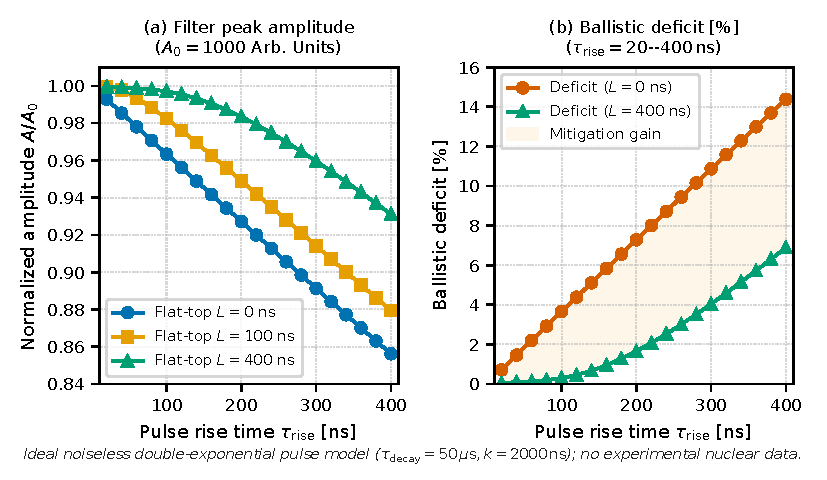
\includegraphics[width=0.85\textwidth]{Img/digital-energy-response.pdf}%
\caption[理想双指数输入下数字梯形滤波响应与弹道亏损缓解特征]{理想双指数输入下数字梯形滤波响应与弹道亏损缓解特征（教学模型，基于附录~F 与 \texttt{ballistic\_deficit\_study.csv} 规范生成，计算参数取 $T_s = 10\text{ ns}$、$\tau_d = 50\ \mu\text{s}$、$\tau_r = 100\text{ ns}$、成形参数 $k = 200$。该曲线展示了不同平顶参数对前沿收集弛豫的平抑效果；注意此处为确定性数值模型输出，未包含探测器连续噪声、电荷收集时间空间非均匀分布及硬件量化限制）。}
\label{fig:5-3-digital-energy-response}
\end{figure}

表~\ref{tab:5-3-ballistic-deficit} 数据表明：延长平顶能够显著压缩不同上升时间引起的幅度差异（例如在 $\tau_r = 220\text{ ns}$ 时，亏损由 $0\text{ ns}$ 平顶的 $8.0030\%$ 降至 $400\text{ ns}$ 平顶的 $2.0735\%$）。但在给定渐近双指数输入与离散取幅规则的本模型中，即使平顶达到 $400\text{ ns}$，依然保留有确定的残余亏损。

第二，极零匹配对平顶形态具有决定性影响。若滤波参数 $M$ 与物理脉冲的衰减时间 $\tau_d$ 存在偏差，平顶区域可能出现斜率或弯曲，不能再按理想平台取幅。此时在名义平顶区间内取幅，测量结果将直接受取样时刻与脉冲到达相位的制约，重新引入测量分散性。

第三，滤波成形参数的选取受到噪声与通过率的双重制约。展宽平顶增加了滤波器的等效积分时间，将增大低频并联噪声在能量提取中的贡献。此外，基底总宽度 $(k + \ell) T_s$ 增加，使后发事件掉入成形时间窗内的概率升高。因此，平顶参数的确定是在弹道亏损平抑、高频与低频噪声折衷以及计数率能力之间寻求的平衡，而非单纯追求单项指标的极限。

\subsection{基线涨落、堆积判弃与核谱强度畸变机制}\label{subsec:5-3-4}

在核反应在束实验环境中，除了孤立脉冲的波形响应外，基线波动、极零失配与事件堆积构成了影响能量估计与能谱强度的关键仪器因素。

前置放大器输出波形通常叠加在一个包含慢漂移的基线上，其来源包括探测器漏电流随环境温度的变化、供电噪声以及远端未分辨脉冲的残留尾部。常用的基线校准方式是在触发脉冲到达之前，利用包含 $N$ 个采样点的无信号区间计算滑动均值~\cite{wu-hongyi-2020-general-purpose-digital-daq-thesis}：
\begin{equation}\label{eq:5-3-bl}
BL = \frac{1}{N} \sum_{m=1}^N v[n_{\text{trig}} - m],
\end{equation}
并在幅度提取时予以扣除。当离散基线采样点满足独立同分布的白噪声假设时，基线估计量的统计方差为 $\sigma_{BL}^2 = \sigma_v^2 / N$。在更一般的实际情形中，滤波与低频漂移会导致采样点之间存在自相关。从成形峰值 $s$ 中减去映射至相同增益刻度的基线估计 $BL$ 后，净幅度的方差满足：
\begin{equation}\label{eq:5-3-var-net}
\mathrm{Var}(s - BL) = \mathrm{Var}(s) + \mathrm{Var}(BL) - 2\mathrm{Cov}(s, BL).
\end{equation}
仅当成形峰值与基线估计相互统计独立且单位映射一致时，总方差才简化为两者的简单平方和。在大事件到达率下，缩短平均窗口 $N$ 会增大基线方差，进而展宽能量分辨率；但若盲目增大 $N$，基线窗极易跨入先前脉冲的衰减尾部，导致基线值被系统性抬高。

极零失配还会留下脉冲后的残差。在本递推与给定指数输入下，采用大于真实匹配值的 $M$ 会产生负残差，反向失配则可留正尾。后续事件可能叠加其上，但最终取幅偏差还取决于基线追踪、扣除、时间位置与判弃逻辑。因此，残差形状和计数率依赖性可用于检验仪器解释，不能直接把某一种残差与所有实现中的固定方向能量偏移对应起来。

为了处理脉冲重叠，数字系统通常采用快慢双滤波通道结构~\cite{wu-hongyi-2020-general-purpose-digital-daq-thesis, wu-2021-general-purpose-digital-daq-waveform-analysis}：
\begin{enumerate}
\item 快通道（触发通道）：采用较短的微分成形参数（成形时间常在百纳秒量级），用于灵敏辨识脉冲前沿并标记事件到达时间。
\item 慢通道（能量通道）：采用成形时间在数微秒量级的精细梯形滤波器，用于滤除噪声并提取脉冲幅度。
\end{enumerate}
在声明的教学实现中，堆积判弃逻辑（PUR）通过快通道的时间标记监测慢通道的成形区间。若在慢通道的特征时间窗内（例如本模型中考查的基底窗口 $(k + \ell) T_s$）检测到第二个脉冲到达，系统将把该事件标记为堆积并予以剔除。在实际硬件固件中，否决窗口的具体形态与逻辑判定取决于具体的探测器与在线配置，并不普遍固定为单一形式。

堆积判弃在滤除变形脉冲、净化全能峰的同时，改变了核谱学的有效计数与事件接受几率。首先，堆积事件被剔除引入了非线性计数损失。对于平均事件率为 $R$ 的泊松过程，时间窗 $\Delta t$ 内至少发生一次后续到达的概率为：
\begin{equation}\label{eq:5-3-pur-poisson}
P(\ge 1; \Delta t) = 1 - e^{-R \Delta t},
\end{equation}
仅在 $R \Delta t \ll 1$ 的低计数率极限下近似表现为正比于窗口长度的线性响应。在在束实验中，当阵列不同角度位置的探测器承受不同计数率时，各通道的事件接受度产生相对差异。若未对各角度通道的有效活时间进行精细校正，将对角分布系数 $W(\theta)$ 与方向角关联（DCO）比值带来测量偏差。其次，在级联跃迁中，若同核相继发射的两个 $\gamma$ 光子在收集时间窗口内同时被同一个晶体吸收（真符合相加），脉冲在物理上直接叠加，当二者无法被单独分辨且均完全沉积能量时，幅度可对应能量和 $E_{\gamma 1}+E_{\gamma 2}$。部分沉积也会改变连续本底与峰计数。真符合相加可造成特定峰的求和损失或其它能量处的求和增加，分支提取须配套相应响应修正。

快触发通道提供的时间标记构成了在束实验符合判定的起点，而亚采样周期定时可采用过零插值恒比定时（CFD）等方法，其在不同信号幅度与采样相位下的时间走动将在第~5.4~节详细推导；而多探测器并发触发、数据缓存区满以及多通道联合活时间损失的定量修正，将在第~5.5~节进行系统分析。
